\documentclass[11pt,a4paper,final]{article} %draft

\usepackage[T1,T2A]{fontenc}
\usepackage[utf8]{inputenc}
\usepackage[english, russian]{babel}

\usepackage[final]{pdfpages}

\usepackage{textcomp,enumitem}

\usepackage{amsmath,amsthm,amssymb}

\usepackage{fancyhdr} % для настройки страницы и колонтитулов

\usepackage{graphicx}

\usepackage{indentfirst} % автоматический отступ в начале каждого раздела

\usepackage[unicode, pdftex, colorlinks, urlcolor=blue]{hyperref}

\usepackage[left=2cm,right=2cm,top=2cm,bottom=2cm,bindingo ffset=0cm]{geometry}

\linespread{1.3} % устанавливает междустрочный интервал

\pagestyle{plain} % для отображения номеров внизу 

\usepackage{float}

\usepackage{listings} 

\usepackage{pdflscape}
\usepackage{listings} 
\definecolor{darkgreen}{rgb}{0,0.5,0}

\lstset{
	backgroundcolor=\color{lightgray!20},   
	basicstyle=\ttfamily\footnotesize\fontfamily{firamono}\selectfont,
	commentstyle=\color{darkgreen},
	keywordstyle=\color{blue},
	numberstyle=\tiny\color{gray},
	stringstyle=\color{red},
	breakatwhitespace=false,
	breaklines=true,
	captionpos=b,
	keepspaces=true,
	numbers=left,
	numbersep=5pt,
	showspaces=false,
	showstringspaces=false,
	showtabs=false,
	tabsize=4,
	language=c++, % Язык программирования
	captionpos=t, % Позиция подписи (b - внизу)
	xleftmargin=0mm, % Отступ слева
	frame=lines, % Тип рамки (single - одинарная, double - двойная, lines - линии)
	framerule=0.25mm, % Толщина рамки
	literate=
	{а}{{\selectfont\char224}}1
	{б}{{\selectfont\char225}}1
	{в}{{\selectfont\char226}}1
	{г}{{\selectfont\char227}}1
	{д}{{\selectfont\char228}}1
	{е}{{\selectfont\char229}}1
	{ж}{{\selectfont\char230}}1
	{з}{{\selectfont\char231}}1
	{и}{{\selectfont\char232}}1
	{й}{{\selectfont\char233}}1
	{к}{{\selectfont\char234}}1
	{л}{{\selectfont\char235}}1
	{м}{{\selectfont\char236}}1
	{н}{{\selectfont\char237}}1
	{о}{{\selectfont\char238}}1
	{п}{{\selectfont\char239}}1
	{р}{{\selectfont\char240}}1
	{с}{{\selectfont\char241}}1
	{т}{{\selectfont\char242}}1
	{у}{{\selectfont\char243}}1
	{ф}{{\selectfont\char244}}1
	{х}{{\selectfont\char245}}1
	{ц}{{\selectfont\char246}}1
	{ч}{{\selectfont\char247}}1
	{ш}{{\selectfont\char248}}1
	{щ}{{\selectfont\char249}}1
	{ъ}{{\selectfont\char250}}1
	{ы}{{\selectfont\char251}}1
	{ь}{{\selectfont\char252}}1
	{э}{{\selectfont\char253}}1
	{ю}{{\selectfont\char254}}1
	{я}{{\selectfont\char255}}1
	{А}{{\selectfont\char192}}1
	{Б}{{\selectfont\char193}}1
	{В}{{\selectfont\char194}}1
	{Г}{{\selectfont\char195}}1
	{Д}{{\selectfont\char196}}1
	{Е}{{\selectfont\char197}}1
	{Ж}{{\selectfont\char198}}1
	{З}{{\selectfont\char199}}1
	{И}{{\selectfont\char200}}1
	{Й}{{\selectfont\char201}}1
	{К}{{\selectfont\char202}}1
	{Л}{{\selectfont\char203}}1
	{М}{{\selectfont\char204}}1
	{Н}{{\selectfont\char205}}1
	{О}{{\selectfont\char206}}1
	{П}{{\selectfont\char207}}1
	{Р}{{\selectfont\char208}}1
	{С}{{\selectfont\char209}}1
	{Т}{{\selectfont\char210}}1
	{У}{{\selectfont\char211}}1
	{Ф}{{\selectfont\char212}}1
	{Х}{{\selectfont\char213}}1
	{Ц}{{\selectfont\char214}}1
	{Ч}{{\selectfont\char215}}1
	{Ш}{{\selectfont\char216}}1
	{Щ}{{\selectfont\char217}}1
	{Ъ}{{\selectfont\char218}}1
	{Ы}{{\selectfont\char219}}1
	{Ь}{{\selectfont\char220}}1
	{Э}{{\selectfont\char221}}1
	{Ю}{{\selectfont\char222}}1
	{Я}{{\selectfont\char223}}1,
	numbers=left, % пронумеровать строки с левой стороны
	breaklines=true % разрешает автоматический перенос строк
}

\hypersetup{
	colorlinks=true, % делает ссылки цветными вместо рамки
	linkcolor=blue, % цвет внутренних ссылок
	urlcolor=blue, % цвет внешних ссылок
	citecolor=blue % цвет ссылок на литературу в тексте
}
\textheight=24cm 
\textwidth=16cm
\oddsidemargin=0pt 
\topmargin=-1.5cm
\parindent=24pt 
\parskip=0pt 
\tolerance=2000 
\flushbottom 

%\usepackage[font=scriptsize]{caption}
\usepackage[labelsep=period]{caption}

\usepackage{amsmath}

\begin{document}
	
\thispagestyle{empty}

\begin{center}
	{\Large МИНОБРНАУКИ РОССИИ}\\
	~\\
	{\large ФЕДЕРАЛЬНОЕ ГОСУДАРСТВЕННОЕ БЮДЖЕТНОЕ ОБРАЗОВАТЕЛЬНОЕ УЧРЕЖДЕНИЕ ВЫСШЕГО ПРОФЕССИОНАЛЬНОГО ОБРАЗОВАНИЯ}\\
	~\\
	{\Large \bf <<САНКТ-ПЕТЕРБУРГСКИЙ ПОЛИТЕХНИЧЕСКИЙ УНИВЕРСИТЕТ ПЕТРА ВЕЛИКОГО>>}\\
	~\\
	{\large Институт компьютерных наук и кибербезопасности }\\
	{\large Высшая школа технологий искусственного интеллекта}\\
	{\large Направление 02.03.01 Математика и компьютерные науки}\\
	~\\
	~\\
	~\\
	~\\
	{\Large \bf  Отчет о выполнении лабораторной работы №6}\\
	\vspace{3mm}
	{\Large {по дисциплине <<Теория графов>>}}\\
	\vspace{3mm}
	{\Large \bf Построение словаря на основе хеш-таблицы и B+-дерева }\\
	~\\
	~\\
	~\\
	~\\
	~\\
	{\large Обучающийся: \underline{\hspace{3.5cm}} \hspace{12mm} Шихалев А.О.}\\
	~\\
	{\large Руководитель: \underline{\hspace{3.5cm}} \hspace{12mm} Востров А.В.}\\
	~\\
	~\\
	~\\
	~\\
\end{center}
\begin{flushright}
	
	«\underline{\hspace{1cm}}»\underline{\hspace{3cm}}20\underline{\hspace{0.7cm}}г.
\end{flushright}
~\\
~\\
~\\
\begin{center}
	{\large Санкт-Петербург, 2024}
\end{center}

\newpage

\tableofcontents

\newpage
\section* {Введение}
\addcontentsline{toc}{section}{Введение}
\par Отчет посвящен разработке приложения-словаря, в котором были реализованы следующие операции: добавление, удаление, поиск, очистка словаря, а также дополнение словаря из текстового файла. Для хранения данных были взяты хэш-таблица и B+-дерево. 

\par Работа была выполнена в среде Visual Studio 2022 на языке программирования С++.
	

\newpage
\section{Математическое описание}
\subsection{Определение хеш-функции}

Хеш-функция — это математическая функция, которая преобразует значение ключа (входные данные произвольного размера) в фиксированное значение, называемое \textbf{хешем} или \textbf{хеш-значением}. Это значение служит для идентификации ключа в структуре данных, чаще всего в хеш-таблицах, или для вычисления адреса хранения данных в памяти или на диске. Основная цель хеш-функции — быстро и эффективно определить место хранения записи по ключу, так как хеш-значение указывает на конкретный адрес (индекс массива, кластер на диске или другой элемент структуры).

Хеш-функция разрабатывается таким образом, чтобы минимизировать вероятность того, что два разных ключа будут иметь одинаковое хеш-значение, но, поскольку мощность множества ключей зачастую значительно больше размера пространства возможных хешей, в большинстве случаев возникает ситуация, когда два или более разных ключа будут иметь одинаковое хеш-значение. Это явление называется \textit{коллизией}.

Важное требование к хеш-функции — равномерное распределение ключей по множеству возможных хеш-значений. При этом множество возможных ключей обычно гораздо больше, чем размер пространства хеш-значений, что делает возникновение коллизий неизбежным. Различные методы хеширования отличаются способами разрешения коллизий (например, метод цепочек, открытая адресация) и способами построения самой хеш-функции (например, метод деления, умножения, криптографические хеш-функции и др.).

\subsection{Полиномиальное хеширование}

\textbf{Полиномиальное хеширование} — это метод вычисления хеш-значения строки, где каждый символ строки рассматривается как коэффициент одночленна в полиноме, а итоговое значение полинома используется для вычисления хеша. Формально, строка $S = s_0 s_1 s_2 \dots s_{n-1}$ хешируется как:

\[
H(S) = (s_0 \cdot a^{n-1} + s_1 \cdot a^{n-2} + \dots + s_{n-1} \cdot a^0) \mod m
\]

где:
\begin{itemize}
	\item $s_i$ — код $i$-го символа строки (например, его числовое значение),
	\item $a$ — некоторое заранее выбранное основание (обычно небольшое простое число, например 33),
	\item $m$ — размер хеш-таблицы или общее количество бакетов.
\end{itemize}

В программе используется упрощенная формула полиномиального хэша: 
\[
\text H(S) = (H(S) \cdot a + s_{i}) \mod m
\]

\subsection{Хеш-таблица}

\textbf{Хеш-таблица} — это структура данных, которая представляет собой одну из реализаций ассоциативной памяти. Она используется для хранения пар вида \texttt{(ключ, значение)} и поддерживает три основные операции: добавление пары, поиск и удаление пары по ключу.

Хеш-таблицы бывают двух основных типов: с открытой адресацией и с использованием метода цепочек (списков). В хеш-таблице с открытой адресацией каждый элемент массива либо содержит пару \texttt{(ключ, значение)}, либо пуст, тогда как в хеш-таблице с цепочками каждый элемент является списком пар, что позволяет хранить несколько пар в одном месте массива. Массив хеш-таблицы состоит из $n$ ячеек, каждая из которых в зависимости от типа может содержать пару или список пар.

Ключевая часть работы хеш-таблицы — это \textbf{хеш-функция}, которая преобразует ключ в индекс массива хеш-таблицы. Важной особенностью является то, что хеш-функция зависит только от ключа и не использует значение. Впрочем, как было указано ранее (см. раздел 1.2), возможны ситуации, при которых различные ключи могут иметь одинаковый хеш — это явление называется \textbf{коллизией}. Для разрешения коллизий используются различные стратегии, такие как линейное пробирование при открытой адресации или хранение нескольких элементов в одной ячейке с помощью списка в методе цепочек.

Одним из важнейших параметров хеш-таблицы является \textbf{коэффициент загрузки}, который равен отношению числа хранимых элементов к количеству ячеек в массиве хеш-таблицы. Этот параметр оказывает значительное влияние на эффективность операций: чем выше коэффициент загрузки, тем больше вероятность коллизий, что может замедлить работу таблицы.

В идеальных условиях, при правильно подобранной хеш-функции и разумном значении коэффициента загрузки, все три основные операции (добавление, поиск и удаление) могут выполняться за время $O(1)$ в среднем. Однако в худшем случае время выполнения может быть значительно больше, особенно если происходит много коллизий. Когда коэффициент загрузки превышает определённый порог, возникает необходимость в \textbf{рехешировании} — процессе, при котором создаётся новый массив большего размера, и все существующие пары из старого массива переносятся в новый, с пересчётом индексов на основе новой хеш-функции.

Структура реализованной хеш-таблицы представлена \hyperref[fig:hash]{риcунке 1} 
\newpage

\begin{figure}[H]
	\centering
	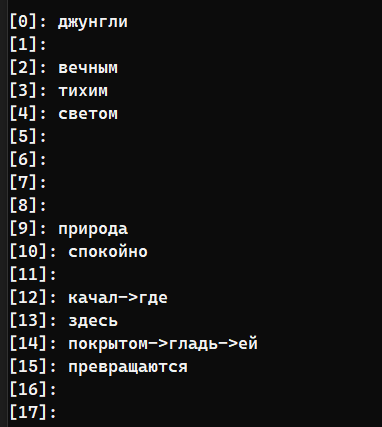
\includegraphics[width=0.5\linewidth]{img/hash.png}
	\caption{Реализованная структура хеш-таблицы}
	\label{fig:hash}
\end{figure}
 

\subsubsection{Разрешение коллизий методом цепочек}

Метод цепочек, или списков, является популярным способом разрешения коллизий в хеш-таблицах. В этом методе каждый элемент массива хеш-таблицы представляет собой связанный список пар \texttt{(ключ, значение)}. Когда несколько ключей хешируются в одно и то же значение (то есть происходит коллизия), все соответствующие пары помещаются в один и тот же список. Как правило, для реализации таких списков используется структура данных, называемая \textbf{односвязным списком}.

Односвязный список — это структура данных, состоящая из узлов, где каждый узел содержит элемент данных и ссылку на следующий узел. Первый элемент списка называют \textit{головой} (head), а последний элемент — \textit{хвостом}. (см. \hyperref[fig:pic1]{рис.2})

\begin{figure}[H]
	\centering
	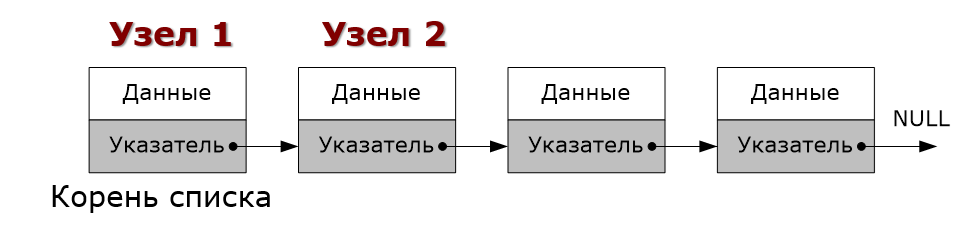
\includegraphics[width=0.8\linewidth]{img/pic1.png}
	\caption{Структура односвязного списка}
	\label{fig:pic1}
\end{figure}

Основное преимущество односвязного списка заключается в том, что его структура позволяет динамически добавлять элементы, при этом элементы в памяти могут располагаться не последовательно, а в произвольном порядке. За счёт этого односвязный список предоставляет гибкость в размере и легко масштабируется. Однако, в отличие от массивов, где доступ к элементам можно получить за постоянное время, в односвязном списке доступ к элементам осуществляется только последовательно.

Когда в методе цепочек при добавлении новой пары возникает коллизия, эта пара добавляется в конец списка, связанного с индексом, на который указала хеш-функция. Время добавления элемента в конец односвязного списка составляет $O(1)$, если есть ссылка на хвост. В противном случае, если список не имеет явного указания на хвост, может потребоваться полный проход по списку, что увеличивает время добавления до $O(n)$, где $n$ — длина списка.

Операции удаления и поиска элемента в односвязном списке требуют последовательного прохода по списку. В худшем случае время поиска или удаления элемента будет $O(n)$, где $n$ — количество элементов в списке. При удалении элемента важно перенаправить ссылки таким образом, чтобы исключить удалённый элемент из цепочки. Это делается путём изменения ссылки предыдущего элемента на следующий после удаляемого узел.

Среднее время выполнения операций в хеш-таблице с цепочками зависит от \textbf{коэффициента загрузки} $\alpha$, который равен отношению количества хранимых элементов к размеру массива. Если распределение хешей равномерное, то средняя длина списка при каждом индексе будет небольшой, и время поиска элемента составит $O(1 + \alpha)$. При низком коэффициенте загрузки ($\alpha \ll 1$) время выполнения операций близко к $O(1)$. Однако при высоком коэффициенте загрузки ($\alpha \gg 1$) длина списков увеличивается, что замедляет операции поиска и удаления, делая их время выполнения ближе к $O(n)$.

\textbf{Операции с односвязным списком}:
\begin{itemize}
	\item \textbf{Добавление элемента} (add): Элемент можно добавить в начало или конец списка. Сложность операции — $O(1)$ при добавлении в начало, $O(1)$ при наличии ссылки на хвост или $O(n)$ без такой ссылки при добавлении в конец.
	\item \textbf{Удаление элемента} (remove): Требуется найти элемент, после чего перенаправить ссылки для исключения узла. Сложность операции — $O(n)$.
	\item \textbf{Поиск элемента} (find): Необходимо последовательно пройти по списку и найти элемент. Сложность операции — $O(n)$.
	\item \textbf{Подсчёт элементов по условию} (count): Проход по списку с проверкой каждого элемента на заданное условие. Сложность операции — $O(n)$.
\end{itemize}


\subsection{B+-дерево}
\textbf{B+-дерево} — это сбалансированная и сильно ветвистая структура данных, предназначенная для эффективного хранения и поиска элементов. Основное преимущество B+-дерева — это возможность выполнения операций поиска, добавления и удаления за $O(\log n)$, где $n$ — количество элементов в дереве.

\textbf{Сбалансированность} означает, что длина путей от корня до любого листа одинакова, что предотвращает деградацию производительности. \textbf{Ветвистость} дерева подразумевает, что каждый узел содержит ссылки на множество потомков, что уменьшает глубину дерева и, следовательно, время выполнения операций.

B+-дерево степени $t > 2$ обладает следующими основными свойствами:
\begin{itemize}
	\item Каждый узел содержит хотя бы один ключ, при этом ключи в узлах упорядочены по возрастанию. Корневой узел содержит от 1 до $2t - 1$ ключей, а все остальные узлы содержат от $t - 1$ до $2t - 1$ ключей.
	\item Листовые узлы не имеют потомков. Внутренние узлы, содержащие $n$ ключей $K_1, K_2, ..., K_n$, имеют $n + 1$ потомков. При этом:
	\begin{itemize}
		\item Первый потомок и все его ключи меньше $K_1$.
		\item Потомки между $K_{i-1}$ и $K_i$ содержат ключи, принадлежащие интервалу $(K_{i-1}, K_i)$ для $2 \leq i \leq n$.
		\item Последний потомок и все его ключи больше $K_n$.
	\end{itemize}
	\item Все листовые узлы находятся на одном уровне, что гарантирует равномерную глубину.
	\item Листовые узлы содержат указатели на своих соседей, что обеспечивает эффективный обход дерева в порядке возрастания ключей.
\end{itemize}

\subsection{Операции над B+-деревом}
\subsubsection{Поиск}
Поиск элемента в B+-дереве начинается с корня и продолжается до листа. Благодаря свойству, что каждый потомок имеет ключи из определённого интервала, можно эффективно направлять поиск. Пусть требуется найти ключ $k$. В каждом внутреннем узле производится одно из следующих действий:
\begin{itemize}
	\item Если $k$ меньше наименьшего ключа узла, спускаемся к первому потомку.
	\item Иначе находим ключи $K_i$, при которых выполняется $K_i \leq k < K_{i+1}$, и спускаемся к $i+1$-му потомку.
	\item Если $k \geq K_n$, спускаемся к последнему потомку.
\end{itemize}
Процесс продолжается до тех пор, пока не будет найден соответствующий лист, который либо содержит ключ $k$, либо указывает на его отсутствие. Поскольку дерево сбалансировано, глубина поиска составляет $O(\log n)$.

\subsubsection{Добавление}
Чтобы добавить новый элемент в B+-дерево, сначала необходимо найти подходящий листовой узел для вставки ключа. Алгоритм добавления следующий:
\begin{itemize}
	\item Если узел не заполнен, то ключ просто добавляется, сохраняя порядок. 
	\item Если узел заполнен (содержит $2t - 1$ ключей), происходит расщепление:
	\begin{itemize}
		\item Узел делится на два, при этом половина ключей переносится в новый узел.
		\item Копия наименьшего ключа из нового узла добавляется в родительский узел.
		\item Если родительский узел также заполнен, процесс расщепления продолжается вверх по дереву.
	\end{itemize}
	\item Если расщепляется корневой узел, создаётся новый корень, содержащий один ключ и две ссылки на потомков.
\end{itemize}
Добавление элемента требует $O(\log n)$ операций, поскольку в худшем случае может потребоваться проход от листа до корня.

\subsubsection{Удаление}
Алгоритм удаления элемента из B+-дерева также начинается с поиска соответствующего листового узла. После нахождения ключа выполняются следующие шаги:
\begin{itemize}
	\item Если после удаления узел остаётся наполовину заполненным (содержит не менее $t - 1$ ключей), операция завершается.
	\item Если узел становится менее чем наполовину заполненным, необходимо перераспределить ключи с соседними узлами. Можно взять ключ у левого или правого «брата» (соседа на том же уровне).
	\item Если перераспределение невозможно, узлы объединяются с соседом, и ключ, указывающий на объединённые узлы, удаляется из родительского узла.
\end{itemize}
Удаление также выполняется за $O(\log n)$, так как может потребоваться корректировка структуры вплоть до корня.

\subsubsection{Пример Б+-дерева}
На \hyperref[fig:pic2]{риcунке 3} представлен пример структуры Б+-дерева. 

\begin{figure}[H]
	\centering
	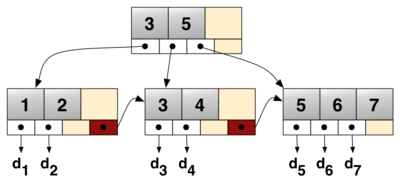
\includegraphics[width=0.7\linewidth]{img/pic2.png}
	\caption{Пример структуры Б+-дерева}
	\label{fig:pic2}
\end{figure}

На \hyperref[fig:tree]{рисунках 4-5} представлена реализованная заполненная структура Б+-дерева.

\begin{figure}[H]
	\centering
	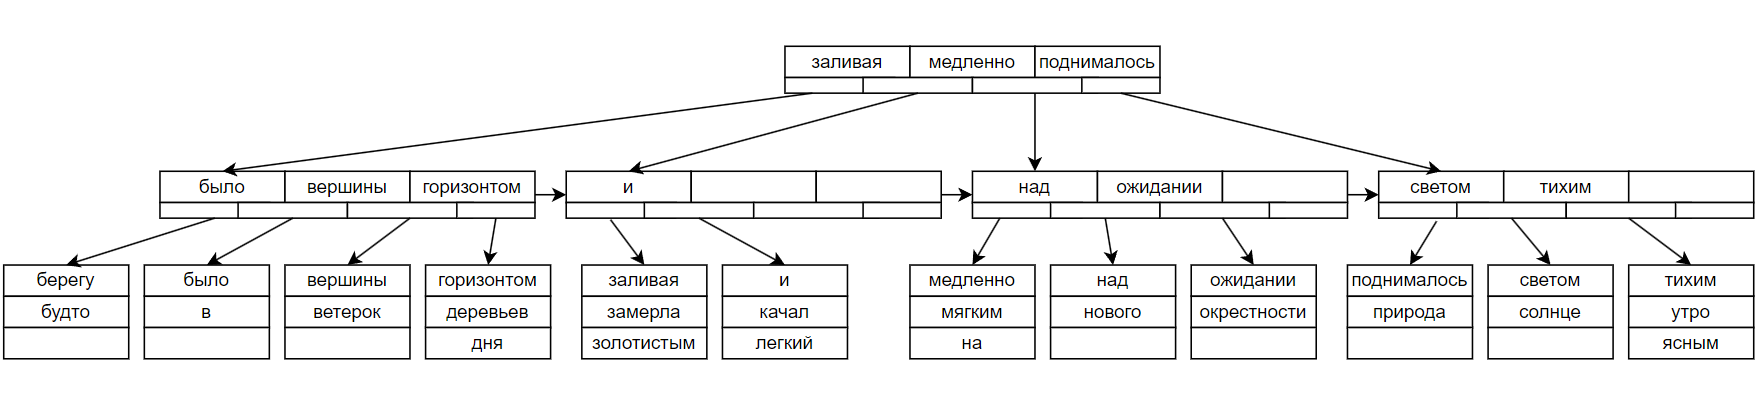
\includegraphics[width=1.05\linewidth]{img/tree.png}
	\caption{Пример реализованной заполненной структуры Б+-дерева}
	\label{fig:tree}
\end{figure}

\begin{figure}[H]
	\centering
	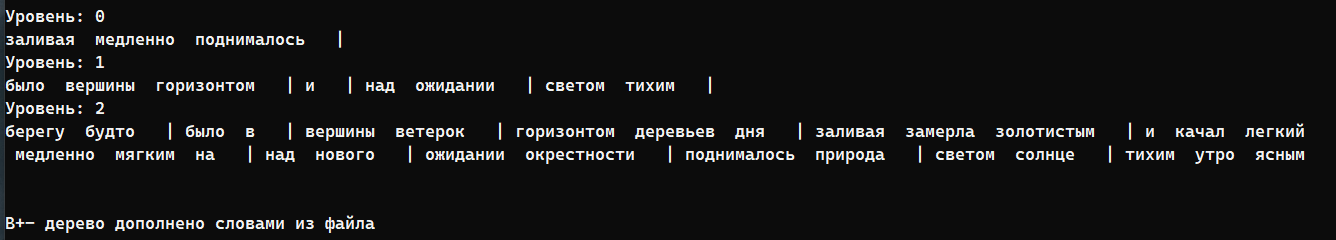
\includegraphics[width=1.1\linewidth]{img/tr.png}
	\caption{Пример реализованной заполненной структуры Б+-дерева}
	\label{fig:tr}
\end{figure}




\newpage
\section{Особенности реализации}
\subsection{Структура Node}
Структура Node представляет из себя реализацию одного узла односвязного списка LinkedList. Структура Node Обладает следующими полями:
\begin{enumerate}
	\item Node* next - указатель на следующий элемент списка.
	\item string data - ключ, слово словаря.
\end{enumerate}

\subsection{Класс LinkedList}
Класс LinkedList представляет из себя реализацию односвязного списка. Класс LinkedList обладает одним полем --- head типа Node*. Это поле является указателем на голову односвязного списка.
  
\subsubsection{Метод insert}
Вход: объект типа LinkedList, string value - строковое значение. \par
Выход: вставленный новый Node в LinkedList. \par

\par Метод \texttt{insert} добавляет новый элемент в конец связного списка. В качестве параметра он принимает строковое значение \texttt{value}, которое должно быть вставлено в список.

\par Этот метод работает за время $O(n)$, где $n$ — количество элементов в списке, так как в худшем случае требуется пройти по всему списку до конца, чтобы вставить новый элемент.

\par Код метода представлен в листинге 1.

\begin{lstlisting}[label=Linkedinsert, caption = Метод insert]
void LinkedList::insert(const string& value) {
	ListNode* newNode = new ListNode(value);
	if (head == nullptr) {
		head = newNode;
	}
	else {
		ListNode* temp = head;
		while (temp->next != nullptr) {
			temp = temp->next;
		}
		temp->next = newNode;
	}
}
\end{lstlisting}

\subsubsection{Метод remove}
Вход: объект типа LinkedList, string key - строковое значение. \par
Выход: bool - true, если элемент был удалён, иначе false. \par

\par Метод \texttt{remove} удаляет элемент из связного списка по его значению \texttt{value}. В случае успешного удаления возвращается \texttt{true}, если элемент не найден — \texttt{false}. 

\par Время работы метода в худшем случае — $O(n)$, где $n$ — количество элементов в списке, так как в худшем случае может потребоваться пройти весь список.

Код метода представлен в листинге 2.
\begin{lstlisting}[label=Linkedremove, caption = Метод remove]
bool LinkedList::remove(const string& value) {
	if (head == nullptr) {
		// cout << "Элемент не найден!" << endl;
		return false;
	}
	
	if (head->data == value) {
		ListNode* temp = head;
		head = head->next;
		delete temp;
		cout << "Слово успешно удалено! " << endl;
		return true;
	}
	
	
	ListNode* current = head;
	ListNode* previous = nullptr;
	
	while (current != nullptr && current->data != value) {
		previous = current;
		current = current->next;
	}
	
	if (current == nullptr) {
		// cout << "Элемент " << value << "не найден!!!" << endl;
		return false;
	}
	
	previous->next = current->next;
	delete current;
	cout << "Слово успешно удалено! " << endl;
	return true;
	
}
\end{lstlisting}

\subsubsection{Метод clear}
Вход: Объект типа LinkedList. \par
Выход: очищенный объект типа LinkedList. \par
Метод производит проход от головы списка до его хвоста, постепенно удаляя на каждом шаге очередной узел.\par
Код метода представлен в листинге 3.
\begin{lstlisting}[label=Linkedclear, caption = Метод clear]
void LinkedList::clear() {
	
	ListNode* current = head;
	while (current != nullptr) {
		ListNode* toDelete = current;
		current = current->next;
		delete toDelete; 
	}
	head = nullptr; 
	
}
\end{lstlisting}

\subsubsection{Метод search}
Вход: объект типа LinkedList, string key - строковое значение. \par
Выход: true, если объект найден, false - если нет. \par

\par Метод \texttt{search} осуществляет поиск элемента по его значению \texttt{value} в связанном списке. Если элемент найден, метод возвращает \texttt{true}, в противном случае — \texttt{false}.

\par Время работы метода в худшем случае — $O(n)$, где $n$ — количество элементов в списке, так как метод может потребовать пройти весь список.

Код метода представлен в листинге 4.
\begin{lstlisting}[label=Linkedclear, caption = Метод find]
bool LinkedList::search(const string& value) {
	ListNode* temp = head;
	
	while (temp != nullptr) {
		if (temp->data == value) {
			return true;
		}
		temp = temp->next;
	}
	return false;
	
}
\end{lstlisting}


\subsection{Класс HashTable}
Класс HashTable представляет из себя реализацию хеш-таблицы. Структура Node Обладает следующими полями:
\begin{enumerate}
	
	\item int total\_buskets - размер массива хеш-таблицы.
	\item int total\_elements - количество элементов в хеш-таблице.
	\item double fillability - коэффициент заполняемости.
	\item LinkedList* table - динамический массив хеш-таблицы.
	
\end{enumerate}

\subsubsection{Метод hashFunction}
Вход: string key - строковое значение. \par
Выход: unsigned int - хеш слова. \par
\par Метод \texttt{hashFunction} вычисляет хеш-значение для строки \texttt{key} с помощью полиномиальной хеш-функции. Эта функция служит для преобразования ключа в числовое значение, которое затем используется для определения индекса в хеш-таблице.

\par Алгоритм работы следующий: метод инициализирует переменную \texttt{hash\_value} равной 0 и использует основание полинома \texttt{a}, равное 33. Для каждого символа строки \texttt{key} хеш-значение обновляется по формуле: \texttt{hash\_value = (hash\_value * a + c) \% total\_buckets}, где \texttt{c} — это числовое значение символа. Операция \texttt{\% total\_buckets} гарантирует, что итоговое значение находится в диапазоне от 0 до \texttt{total\_buckets - 1}, что предотвращает выход за пределы массива.

Код метода представлен в листинге 5.
\begin{lstlisting}[label=hashCode, caption = Метод hashFunction]
unsigned int HashTable::hashFunction(const string& key) {
	
	unsigned int hash_value = 0;
	int a = 33; // основание полинома
	
	for (char c : key) {
		hash_value = (hash_value * a + static_cast<unsigned int>(c)) % total_buckets;
	}
	
	return hash_value;
}
\end{lstlisting}

\subsubsection{Метод insert}
Вход: объект типа HashTable, string key - строковое значение. \par
Выход: вставленный обьект в хеш-таблицу. 

\par Метод \texttt{insert} добавляет новый элемент с ключом \texttt{key} в хеш-таблицу. Процесс начинается с вычисления индекса для ключа с помощью хеш-функции \texttt{hashFunction(key)}. Если ключ уже существует в таблице (проверка выполняется с помощью метода \texttt{search}), добавление не выполняется. 

\par Если элемент отсутствует, вызывается метод вставки в связанный список, хранящийся в соответствующем индексе хеш-таблицы. После этого обновляется количество элементов и вычисляется коэффициент заполненности таблицы (\texttt{fillability}), как отношение общего числа элементов к числу бакетов.

\par Если коэффициент заполненности превышает 0.9, выполняется процедура \texttt{rehash}, которая пересчитывает хеш-таблицу с большим количеством бакетов для предотвращения переполнения и повышения эффективности.


Код метода представлен в листинге 6.
\begin{lstlisting}[label=add, caption = Метод insert]
void HashTable::insert(const string& key) {
	int index = hashFunction(key);
	if (search(key) == -1) {
		table[index].insert(key);
		total_elements++;
		fillability = static_cast<double>(total_elements) / static_cast<double>(total_buckets);
	}
	if (fillability >= 0.9) {
		rehash();
	}
}
\end{lstlisting}

\subsubsection{Метод remove}
Вход: объект типа HashTable, string key\_r - строковое значение. \par
Выход: удаленный объект. \par

\par Метод \texttt{remove} удаляет элемент с указанным ключом \texttt{key} из хеш-таблицы. Сначала вычисляется индекс с помощью хеш-функции \texttt{hashFunction(key)}. Затем вызывается метод удаления \texttt{remove} для связанного списка, который хранится в этом индексе.

\par Если удаление прошло успешно, количество элементов уменьшается, и коэффициент заполненности таблицы \texttt{fillability} пересчитывается. Если элемент с таким ключом не был найден, выводится сообщение об ошибке.

\par Время работы метода удаления в среднем — $O(1)$, если коллизий мало. В худшем случае, если в таблице много коллизий, время работы увеличивается до $O(n)$, где $n$ — длина связанного списка.

Код метода представлен в листинге 7.

\begin{lstlisting}[label=remove, caption = Метод remove]
void HashTable::remove(const string& key) {
	
	int index = hashFunction(key);
	if (table[index].remove(key)) {
		total_elements--;
		fillability = static_cast<double>(total_elements) / static_cast<double>(total_buckets);
	}
	
	else cout << "\n Элемент не найден! " << endl;
}
\end{lstlisting}


\subsubsection{Метод clear}
Вход: объект типа HashTable. \par
Выход: очищенный массив. \par

\par Метод \texttt{clear} очищает все элементы хеш-таблицы. Он проходит по всем корзинам \texttt{total\_buckets} и вызывает метод \texttt{clear} для каждого связанного списка, тем самым удаляя все элементы, хранящиеся в этих списках.

\par После этого количество элементов в таблице \texttt{total\_elements} устанавливается в 0, а коэффициент заполненности \texttt{fillability} обнуляется.

Код метода представлен в листинге 8.

\begin{lstlisting}[label=Linkedclear, caption = Метод clear]
void HashTable::clear() {
	for (int i = 0; i < total_buckets; i++) {
		table[i].clear();
	}
	total_elements = 0;
	fillability = 0.0;
	cout << "Хэш-таблица полностью очищена!" << endl;

}
\end{lstlisting}

\subsubsection{Метод search}
Вход: Объект типа HashTable, string key - строковое значение. \par
Выход: индекс бакета в случае, если элемент найден или -1, если не найден. 

\par Метод \texttt{search} выполняет поиск ключа в хеш-таблице и возвращает индекс корзины, в которой был найден ключ. Если ключ найден, метод возвращает индекс корзины, соответствующий этому ключу. Если ключ отсутствует в таблице, метод возвращает \texttt{-1}.

\par Для поиска ключа сначала вычисляется индекс корзины с помощью хеш-функции \texttt{hashFunction}. Затем метод проверяет наличие ключа в корзине по этому индексу с помощью метода \texttt{search} класса \texttt{LinkedList}. Если ключ найден, метод возвращает индекс корзины, в противном случае возвращается \texttt{-1}.

\par Время выполнения метода зависит от количества элементов в корзине и составляет $O(1)$ в среднем случае при равномерном распределении ключей.


Код метода представлен в листинге 9.
\begin{lstlisting}[label=find, caption = Метод find]
int HashTable::search(const string& key) {
	
	int index = hashFunction(key);
	if (table[index].search(key)) return index;
	else return -1;
	
}
\end{lstlisting}

\subsubsection{Метод insertFromFile}
Вход: объект типа HashTable, string filename - название файла в строковом формате. \par
Выход: дополненная хеш-таблица. \par

\par Метод \texttt{insertFromFile} отвечает за добавление элементов в хеш-таблицу из файла. Вначале открывается файл для чтения. Если файл не удалось открыть, выводится сообщение об ошибке.

\par Далее, метод построчно считывает файл, разбивая каждую строку на слова. Каждое слово преобразуется в нижний регистр и очищается от неалфавитных и нечисловых символов. После этого, если слово не пустое, оно добавляется в хеш-таблицу с помощью метода \texttt{insert}.

Код метода представлен в листинге 10.

\begin{lstlisting}[label=loadFromFile, caption = Метод insertFromFile]
void HashTable::insertFromFile(const string& filename) {
	ifstream file(filename);
	if (!file.is_open()) {
		cout << "Ошибка! Не удалось открыть файл!" << filename << endl;
		return;
	}
	string line, word;
	while (getline(file, line)) {
		stringstream ss(line);
		while (ss >> word) {
			transform(word.begin(), word.end(), word.begin(), ::tolower);
			word.erase(remove_if(word.begin(), word.end(), [](char c) {
				return !isAlphaNum(c);
			}), word.end());
			
			if (!word.empty()) { 
				insert(word);
				// cout << "Добавили " << word << endl;
			}
		}
	}
	// cout << "Количество элементов: " << total_elements << endl;
	// cout << "Коэф. заполняемости хэш-таблицы: " << fillability << endl;
}
\end{lstlisting}

\subsubsection{Метод rehash}
Вход: объект типа HashTable, total\_buckets - количество бакетов в хеш-таблице \par
Выход: дополненная хеш-таблица. \par

\par Метод \texttt{rehash} выполняет процесс пересоздания хеш-таблицы с увеличением числа корзин. Сначала старое количество корзин сохраняется в переменной \texttt{old\_buckets}, и количество корзин удваивается. Затем создается новый массив корзин с обновленным размером.

\par Все элементы из старой таблицы переносится в новый массив. Для этого метод перебирает все корзины старой таблицы и вставляет все содержащиеся в них элементы в новую таблицу, используя метод \texttt{insert}.

\par После переноса всех элементов старая таблица удаляется, освобождая память.

\par Время выполнения метода зависит от количества элементов в таблице и составляет $O(n)$, где $n$ — количество элементов в таблице до выполнения операции \texttt{rehash}.

Код метода представлен в листинге 11.

\begin{lstlisting}[label=HashRehash, caption = Метод rehash]
	void HashTable::rehash() {
		
		// cout << "Пересоздаем таблицу..." << endl;
		
		int old_buckets = total_buckets;
		
		total_buckets *= 2;
		
		LinkedList* old_table = table; 
		table = new LinkedList[total_buckets];
		total_elements = 0;
		
		for (int i = 0; i < old_buckets; i++) {
			
			ListNode* temp = old_table[i].getHead();
			
			while (temp != nullptr) {
				insert(temp->data);
				temp = temp->next;
			}
			
		}
		
		delete[] old_table;
		
	}
\end{lstlisting}



\subsection{Класс Node}
Класс Node является базовой реализацией узла B+-дерева. Этот класс обладает следующими полями:
\begin{enumerate}
	\item InterNode* Parent --- указатель на родителя.
	\item vector<string> key --- массив ключей.
	\item int count --- количество ключей в узле.
	\item bool isLeaf --- true, если является листом, иначе false.
\end{enumerate}

\subsubsection{Метод GetBrother}
Вход: объект типа Node, int\& flag - ссылка на целочисленное значение. \par
Выход: указатель на объект типа Node. \par
Первым делом метод проверяет, является ли текущий узел корнем. Если им является, то возвращается нулевой указатель. Иначе производится проход по всем детям родительского узла, пока не будет найден текущий узел. Далее проводится проверка: если текущий узел является самым правым дочерним узлом, то из метода возвращается указатель на левый узел и в переменную flag устанавливается значение 1, иначе возвращается указатель на правый узел и в переменную flag устанавливается значение 2. \par
Код метода представлен в листинге 12.
\begin{lstlisting}[label=GetBrother, caption = Метод GetBrother]
	Node* Node::GetBrother(int& flag) {
		if (Parent == NULL)
		return NULL;
		
		Node* p = NULL;
		for (int i = 0; i <= Parent->count; i++) {
			if (Parent->Child[i] == this) {
				if (i == Parent->count) {
					p = Parent->Child[i - 1];
					flag = 1;
				}
				else {
					p = Parent->Child[i + 1];
					flag = 2;
				}
			}
		}
		return p;
	}
\end{lstlisting}


\subsection{Класс LeafNode}
Класс InterNode является реализацией листового узла B+-дерева. Он наследует класс Node. Этот класс обладает дополнительными полями LeafNode* Pre\_Node - указатель на лист слева, Next\_Node - указатель на лист справа. 

\subsubsection{Метод Split}
Вход: Объект типа LeafNode, p - указатель на узел типа LeafNode. \par
Выход: значение наименьшего ключа узла p\par
Первым делом метод производит перенос M последних ключей в лист p, после чего обновляет счётчик количества элементов в текущем узле и в правом брате. Далее возвращает значение наименьшего ключа узла p. \par
Код метода представлен в листинге 13.
\begin{lstlisting}[label=Split, caption = Метод Split]
	string LeafNode::Split(LeafNode* p) {
		int j = 0;
		for (int i = M - 1; i < M * 2 - 1; i++, j++) 
		p->key[j] = this->key[i];
		
		this->count = this->count - j;
		p->count = j;
		return p->key[0];
	}
\end{lstlisting}

\subsubsection{Метод Insert}
Вход: объект типа LeafNode, string value - строковое значение. \par
Выход: true, если ключ записан, false, если нет. \par
Первым делом метод производит поиск позиции, куда будет записан ключ. После чего перемещает ключи справа от этой позиции вправо на 1 ячейку. Далее записывает на позицию ключ value. В конце возвращает true. \par
Код метода представлен в листинге 14.
\begin{lstlisting}[label=Insert, caption = Метод Insert]
	bool LeafNode::Insert(string value) {
		int i = 0;
		for (; (value > key[i]) && (i < count); i++);
		
		for (int j = count; j > i; j--)
		key[j] = key[j - 1];
		
		key[i] = value;
		count++;
		return true;
	}
\end{lstlisting}

\subsubsection{Метод Delete}
Вход: объект типа LeafNode, string value - строковое значение. \par
Выход: true, если элементы сместились, false, если ключ не найден. \par
Первым делом метод производит поиск ключа в листе, если ключа не было найдено, то возвращает false. Иначе все элементы справа от позиции найденного ключа смещаются влево на 1. После чего метод возвращает true. \par
Код метода представлен в листинге 15.
\begin{lstlisting}[label=Delete, caption = Метод Delete]
	bool LeafNode::Delete(string value)
	{
		bool found = false;
		int i = 0;
		for (; i < count; i++) {
			if (value == key[i]) {
				found = true;
				break;
			}
		}
		if (found == false)
		return false;
		int j = i;
		for (; j < count - 1; j++)
		key[j] = key[j + 1];
		key[j] = "";
		count--;
		return true;
	}
\end{lstlisting}

\subsubsection{Метод Merge}
Вход: объект типа LeafNode, указатель на узел типа LeafNode. \par
Выход: true, если вставка ключей произошла успешно, иначе false. \par
Изначально метод проверяет, чтобы после слияния количество элементов было больше M*2, если это так, то производится вставка всех ключей брата в текущий узел методом Insert и возвращается true, иначе возвращается false.\par
Код метода представлен в листинге 16.
\begin{lstlisting}[label=Merge, caption = Метод Merge]
	bool LeafNode::Merge(LeafNode* p) {
		if (this->count + p->count > M * 2 - 1) 
		return false;
		for (int i = 0; i < p->count; i++)
		this->Insert(p->key[i]);
		return true;
	}
\end{lstlisting}




\subsection{Класс InterNode}
Класс InterNode является реализацией внутреннего узла B+-дерева. Он наследует класс Node. Этот класс обладает дополнительным полем vector<Node*> Child - это массив указателей на детей этого узла.

\subsubsection{Метод Merge}
Вход: объект типа InterNode, указатель на узел типа InterNode. \par
Выход: bool значение - результат выполнения операции слияния. \par
Первым делом метод размещает наибольший ключ крайнего левого ребёнка правого брата на последнюю позицию в списке ключей текущего узла. После этого он метод перемещает указатель на крайнего левого ребёнка правого брата в конец списка детей текущего узла. После этого в цикле перемещает оставшиеся ключи и оставшихся детей правого брата в правую часть списка ключей и списка детей текущего узла. После этого возвращается true. \par
Код метода представлен в листинге 17.
\begin{lstlisting}[label=Merge, caption = Метод Merge]
	bool InterNode::Merge(InterNode* p) {
		key[count] = p->Child[0]->key[0];
		count++;
		Child[count] = p->Child[0];
		Child[count]->Parent = this;
		for (int i = 0; i < p->count; i++) {
			key[count] = p->key[i];
			count++;
			Child[count] = p->Child[i + 1];
			Child[count]->Parent = this;
		}
		return true;
	}
\end{lstlisting}

\subsubsection{Метод Insert}
Вход: объект типа InterNode, string value - строковое значение; указатель на узел типа Node. \par
Выход: bool значение - результат выполнения операции вставки. \par
Первым циклом производится поиск позиции, куда будет добавлен ключ и ребёнок. Следующим циклом производится перемещение ключей на единицу вправо от найденной позиции. Аналогично делается и для детей. После этого в найденную позицию записывается ключ и правым ребёнком этого ключа записывается узел New. \par
Код метода представлен в листинге 18.
\begin{lstlisting}[label=Insert, caption = Метод Insert]
	bool InterNode::Insert(string value, Node* New) {
		int i = 0;
		for (; (i < count) && (value > key[i]); i++);
		
		for (int j = count; j > i; j--)
		key[j] = key[j - 1];
		
		for (int j = count + 1; j > i + 1; j--)
		Child[j] = Child[j - 1];
		
		key[i] = value;
		Child[i + 1] = New;
		New->Parent = this;
		count++;
		return true;
	}
\end{lstlisting}


\subsubsection{Метод Split}
Вход: объект типа InterNode, указатель на узел типа InterNode, string k - строковое значение. \par
Выход: строковое значение. \par
Изначально производится вычисление индекса, по которому будет производиться деление узла на две части. Этот индекс равен M-1, то есть M-1 элементов останутся в текущем узле, а последние M - 1 ключей переместятся в новый узел. Следует заметить, что оставшийся ключ записывается в переменную k. Также происходит и с детьми текущего узла. Далее возвращаем ключ k. \par
Код метода представлен в листинге 19.
\begin{lstlisting}[label=Split, caption = Метод Split]
	string InterNode::Split(InterNode* p, string k) {
		int i = 0, j = 0;
		
		int pos = M-1;
		k = this->key[pos];
		j = 0;
		for (i = pos + 1; i < M * 2 - 1; i++, j++)  
		p->key[j] = this->key[i];
		j = 0;
		for (i = pos + 1; i <= M * 2 - 1; i++, j++) { 
			this->Child[i]->Parent = p;
			p->Child[j] = this->Child[i];
		}
		this->count = pos; 
		p->count = M * 2 - pos - 2; 
		return k;
	}
\end{lstlisting}


\subsubsection{Метод Delete}
Вход: объект типа InterNode, string k - строковое значение. \par
Выход: bool значение - результат выполнения операции удаления. \par
Производим поиск позиции, где расположен ключ, далее удаляем ключ. после чего удаляем ребёнка справа от этого ключа. \par
Код метода представлен в листинге 20.
\begin{lstlisting}[label=Delete, caption = Метод Delete]
	bool InterNode::Delete(string k) {
		int i = 0;
		for (; (k >= key[i]) && (i < count); i++);
		
		for (int j = i - 1; j < count - 1; j++)
		key[j] = key[j + 1];
		
		int d = i;
		for (; d < count; d++) {
			Child[d] = Child[d + 1];
		}
		Child[d] = NULL;
		count--;
		return true;
	}
\end{lstlisting}


\subsubsection{Метод Slib}
Вход: объект типа InterNode, указатель на узел типа InterNode. \par
Выход: bool значение - результат выполнения операции переноса. \par
Первым делом проверяем на какого брата указывает p, если левый, то переносим из левого брата наибольшего ребёнка в текущий узел на позицию наименьшего ребёнка. Иначе из правого брата переносим наименьшего ребёнка на позицию старшего ребёнка текущего узла, после чего у старшего брата сдвигаем ключи и детей на один влево. \par
Код метода представлен в листинге 21.
\begin{lstlisting}[label=Slib, caption = Метод Slib]
	bool InterNode::Slib(InterNode* p) {
		int i, j;
		if (p->key[0] < this->key[0]) {
			for (i = count; i > 0; i--)
			key[i] = key[i - 1];
			for (j = count + 1; j > 0; j--)
			Child[j] = Child[j - 1];
			key[0] = Child[0]->key[0];
			Child[0] = p->Child[p->count];
			Child[0]->Parent = this;
		}
		else {
			key[count] = p->Child[0]->key[0];
			Child[count + 1] = p->Child[0];
			Child[count + 1]->Parent= this;
			for (i = 1; i < p->count; i++)
			p->key[i - 1] = p->key[i];
			for (j = 0; j < p->count; j++)
			p->Child[j] = p->Child[j + 1];
		}
		this->count++;
		p->count--;
		return true;
	}
\end{lstlisting}

\subsection{Класс Bplus}
Класс Bplus является реализацией B+-дерева. Он обладает следующими полями:
\begin{enumerate}
	\item int M - ранг дерева.
	\item Node* Root - указатель на корень дерева.
\end{enumerate}

\subsubsection{Метод Find}
Вход: объект типа BPlus, string data - строковое значение. \par
Выход: указатель на узел типа LeafNode. \par
Метод начинает свою работу с корня дерева p. Пробегается по всем ключам корня, пока не находит ключ в узле, больший ключа data. Как только такой ключ будет найден, указатель на ребёнка справа от этого узла будет записан в переменную p. После чего всё повторяется. Так будет продолжаться, пока не будет достигнуть лист. \par
Код метода представлен в листинге 22.
\begin{lstlisting}[label=Find, caption = Метод Find]
	LeafNode* Bplus::Find(string data) {
		int i = 0;
		Node* p = Root;
		InterNode* q;
		
		while (NULL != p) {
			if (p->isLeaf)
			break;
			for (i = 0; i < p->count; i++) {
				if (data < p->key[i])
				break;
			}
			q = (InterNode*)p;
			p = q->Child[i];
		}
		return (LeafNode*)p;
	}
\end{lstlisting}

\subsubsection{Метод Add\_Node}
Вход: объект типа BPlus, p - указатель на узел типа InterNode, k - строковое значение, New\_Node - указатель на узел типа Node. \par
Выход: bool значение - результат выполнения операции добавления узла \par
Первоначально производится проверка на существование узла p, а также на то, чтобы он не был листовым узлом. Далее проверяем, если количество копий ключей в узле меньше M * 2 - 1, то можем добавить в этот узел ключ k. Иначе производим расщепление текущего узла на два. Далее определяем, в какой узел будет помещён ключ с ребёнком, помещаем в выбранный узел. Далее, если текущий узел уже является корневым, то создаём расширяем дерево вверх, иначе снова вызываем метод Add\_Node для родителя. \par
Код метода представлен в листинге 23.
\begin{lstlisting}[label=AddNode, caption = Метод Add\_Node]
	bool Bplus::Add_Node(InterNode* p, string k, Node* New_Node) {
		if (p == NULL || p->isLeaf)
		return false;
		if (p->count < M * 2 - 1) 
		return p->Insert(k, New_Node);
		
		InterNode* Brother = new InterNode(M);
		string NewKey = p->Split(Brother, k);
		
		if (Brother->Child[0]->key[0] < k) {
			Brother->Insert(k, New_Node);
		}
		else {
			p->Insert(k, New_Node);
		}
		
		InterNode* parent = (InterNode*)(p->Parent);
		if (parent == NULL) {
			parent = new InterNode(M);
			parent->Child[0] = p;
			parent->key[0] = NewKey;
			parent->Child[1] = Brother;
			p->Parent = parent;
			Brother->Parent = parent;
			parent->count = 1;
			Root = parent;
			return true;
		}
		return Add_Node(parent, NewKey, Brother);
	}
\end{lstlisting}

\subsubsection{Метод Search}
Вход: объект типа Bplus, string data - строковое значение. \par
Выход: bool значение; модификация строки sPath. \par
Метод производит действия, аналогичные методу Find, однако не останавливается на нахождении листового узла. Он проходится по листовому узлу в поисках ключа, если находит, то строка из метода будет возвращено значение true, иначе false. Также по мере спуска по дереву, метод записывает переход с одного яруса дерева на другой в переменную по ссылке sPath. \par
Код метода представлен в листинге 24.
\begin{lstlisting}[label=Search, caption = Метод Search]
	bool Bplus::Search(string data) {
		int i = 0;
		Node* p = Root;
		if (p == NULL)
		return false;
		InterNode* q;
		while (p != NULL) {
			if (p->isLeaf)
			break;
			for (i = 0; (i < p->count) && (data >= p->key[i]); i++);
			int k = i > 0 ? i - 1 : i;
			q = (InterNode*)p;
			p = q->Child[i];
		}
		if (p == NULL)
		return false;
		bool found = false;
		for (i = 0; i < p->count; i++) {
			if (data == p->key[i])
			found = true;
		}
		return found;
	}
\end{lstlisting}


\subsubsection{Метод Insert}
Вход: объект типа Bplus, string data - строковое значение. \par
Выход: bool значение - результат выполнения операции вставки. \par
Метод изначально производит проверку на наличие ключа в дереве, если он есть, то метод возвращает false. Далее производится поиск листового узла, где ключ можно было бы разместить. Если такой не был найден, это означает, что дерево ещё пустое, поэтому создаётся корневой узел дерева. Далее, если размер текущего узла меньше M*2 - 1, то вставляет данные в этот узел. Иначе требуется расщепить его, используя метод Split класса LeafNode, который возвращает ключ, который в дальнейшем потребуется для изменения данных в родителе. После расщепления происходит переприсваивание ссылок на левых/правых братьев. Далее выбирается, в какой листовой узел будет размещён конкретный ключ. Далее требуется проверить, что если произошло расщепление корневого узла, то требуется создать новый узел. Иначе производится обновление ключа в узлах-родителях. \par
Код метода представлен в листинге 25.
\begin{lstlisting}[label=Insert, caption = Метод Insert]
	bool Bplus::Insert(string data) {
		string a;
		if (Search(data, a) == true)
		return false;
		
		LeafNode* Old_Node = Find(data);
		
		if (NULL == Old_Node) {
			Old_Node = new LeafNode(M);
			Root = Old_Node;
		}
		
		if (Old_Node->count < M * 2 - 1)
		return Old_Node->Insert(data);
		
		LeafNode* New_Node = new LeafNode(M);
		
		string k = Old_Node->Split(New_Node);
		
		LeafNode* OldNext = Old_Node->Next_Node;
		Old_Node->Next_Node = New_Node;
		New_Node->Next_Node = OldNext;
		New_Node->Pre_Node = Old_Node;
		
		if (OldNext != NULL)
		OldNext->Pre_Node = New_Node;
		
		if (data < k) {
			Old_Node->Insert(data);
		}
		else {
			New_Node->Insert(data);
		}
		InterNode* parent = (InterNode*)(Old_Node->Parent);
		
		if (parent == NULL) {
			InterNode* New_Root = new InterNode(M);
			New_Root->Child[0] = Old_Node;
			New_Root->key[0] = k;
			New_Root->Child[1] = New_Node;
			Old_Node->Parent = New_Root;
			New_Node->Parent = New_Root;
			New_Root->count = 1;
			Root = New_Root;
			return true;
		}
		
		return Add_Node(parent, k, New_Node);
	}
\end{lstlisting}

\subsubsection{Метод Delete}
Вход: объект типа Bplus, string data - строковое значение. \par
Выход: bool значение - результат выполнения операции удаления. \par
Первым делом метод производит поиск листового узла, в котором может быть расположен ключ. Далее производится удаление ключа из узла. После этого метод получает ссылку на родителя этого листового узла. Далее, проверяем ситуацию, если родитель у текущего узла нет, то требуется проверить, не был ли элемент последним в листовом узле, если был, то удаляем этот листовой узел. Далее, если количество ключей до сих пор больше M-1, то пробуем обновить ключи в родителе и возвращаем true. Если же узел меньше M-1, то пробуем переместить ключ от левого брата или ключ от правого брата. Если же и это не получилось сделать, то это значит, что можно произвести слияние текущего узла с одним из братьев. Далее алгоритм производит слияние узлов и вызывает метод Remove\_Node, который будет удалять ключ data по направлению к корню дерева. \par
Код метода представлен в листинге 26.
\begin{lstlisting}[label=Delete, caption = Метод Delete]
	bool Bplus::Delete(string data) {
		LeafNode* Old_Node = Find(data);
		string NewKey = Old_Node->key[0];
		if (Old_Node == NULL)
		return false;
		if (false == Old_Node->Delete(data))
		return false;
		
		InterNode* parent = (InterNode*)(Old_Node->Parent);
		if (NULL == parent || parent->Child.size() == 0) {
			if (0 == Old_Node->count) {
				delete Old_Node;
				Root = NULL;
			}
			return true;
		}
		if (Old_Node->count >= M - 1) {
			for (int i = 0; (i < parent->count) && (data >= parent->key[i]); i++) {
				if (parent->Child[i + 1]->isLeaf) {
					parent->key[i] = parent->Child[i + 1]->key[0];
				}
				else {
					parent->key[i] = static_cast<InterNode*>(parent->Child[i + 1])->getMin();
				}
			}
			return true;
		}
		
		int flag = 1;
		LeafNode* Brother = (LeafNode*)(Old_Node->GetBrother(flag));
		string NewData = "";
		if (Brother->count > M - 1) { 
			if (1 == flag) {
				NewData = Brother->key[Brother->count - 1];
			}
			else {
				NewData = Brother->key[0];
			}
			Old_Node->Insert(NewData);
			Brother->Delete(NewData);
			
			if (1 == flag) {
				for (int i = 0; i <= parent->count; i++) {
					if (parent->Child[i] == Old_Node && i > 0)
					parent->key[i - 1] = Old_Node->key[0];
				}
			}
			else {
				for (int i = 0; i <= parent->count; i++) {
					if (parent->Child[i] == Old_Node && i > 0)
					parent->key[i - 1] = Old_Node->key[0];
					if (parent->Child[i] == Brother && i > 0)
					parent->key[i - 1] = Brother->key[0];
				}
			}
			return true;
		}
		
		if (1 == flag) {
			Brother->Merge(Old_Node);
			NewKey = Old_Node->key[0];
			LeafNode* OldNext = Old_Node->Next_Node;
			Brother->Next_Node = OldNext;
			if (NULL != OldNext)
			OldNext->Pre_Node = Brother;
			delete Old_Node;
		}
		else {
			Old_Node->Merge(Brother);
			NewKey = Brother->key[0];
			LeafNode* OldNext = Brother->Next_Node;
			Old_Node->Next_Node = OldNext;
			if (NULL != OldNext)
			OldNext->Pre_Node = Old_Node;
			
			delete Brother;
		}
		return Remove_Node(parent, NewKey);
	}
\end{lstlisting}

\subsubsection{Метод Remove\_Node}
Вход: объект типа Bplus, указатель на узел типа InterNode*, string k - строковое значение. \par
Выход: bool значение - результат выполнения операции удаления узла. \par
Изначально метод попробует удалить ключ из текущего узла, если не получилось, значит такого ключа больше нет по направлению к корню дерева и метод можно завершать со значением false. Далее производятся те же действия, что и в методе Delete, за исключением последней части, где при слиянии с братьями не производится установка ссылок друг на друга, т.к. во внутренних узлах их нет. \par
Код метода представлен в листинге 27.
\begin{lstlisting}[label=RemoveNode, caption = Метод Remove\_Node]
	bool Bplus::Remove_Node(InterNode* p, string k) {
		if (k == "")
		return false;
		
		if (false == p->Delete(k))
		return false;
		
		InterNode* parent = (InterNode*)(p->Parent);
		if (NULL == parent || parent->Child.size() == 0) {
			if (0 == p->count) {
				Root = p->Child[0];
				delete p;
			}
			return true;
		}
		
		if (p->count >= M - 1) { 
			for (int i = 0; (i < parent->count) && (k >= parent->key[i]); i++) { // обновляем ключи в родителе если надо
				if (parent->key[i] == k)
				parent->key[i] = p->getMin();
			}
			for (int i = 0; i < p->count; i++) { // обновляем ключи в узле относительно правого ребенка
				if (p->Child[i + 1]->isLeaf) {
					p->key[i] = p->Child[i + 1]->key[0];
				}
				else {
					p->key[i] = static_cast<InterNode*>(p->Child[i + 1])->getMin();
				}
			}
			
			return true;
		}
		int flag = 1;
		InterNode* Brother = (InterNode*)(p->GetBrother(flag));
		if (Brother->count > M - 1) {
			p->Slib(Brother);
			
			for (int i = 0; i < Brother->count; i++) { // обновляем ключи у узла, откуда перенесли
				if (Brother->Child[i + 1]->isLeaf) {
					Brother->key[i] = Brother->Child[i + 1]->key[0];
				}
				else {
					Brother->key[i] = static_cast<InterNode*>(Brother->Child[i + 1])->getMin();
				}
			}
			for (int i = 0; i < p->count; i++) { // обновляем ключи у узла, куда перенесли
				if (p->Child[i + 1]->isLeaf) {
					p->key[i] = p->Child[i + 1]->key[0];
				}
				else {
					p->key[i] = static_cast<InterNode*>(p->Child[i + 1])->getMin();
				}
			}
			for (int i = 0; i <= parent->count; i++) {  // обновляем ключи у родителя
				if (parent->Child[i] == p && i > 0)
				parent->key[i - 1] = p->getMin();
				if (parent->Child[i] == Brother && i > 0)
				parent->key[i - 1] = Brother->getMin();
			}
			return true;
		}
		string NewKey = "";
		if (1 == flag) {
			Brother->Merge(p);
			for (int i = 0; i < Brother->count; i++) { // обновляем ключи в узле
				if (Brother->Child[i + 1]->isLeaf) {
					Brother->key[i] = Brother->Child[i + 1]->key[0];
				}
				else {
					Brother->key[i] = static_cast<InterNode*>(Brother->Child[i + 1])->getMin();
				}
			}
			NewKey = p->key[0];
			delete p;
		}
		else {
			p->Merge(Brother);
			for (int i = 0; i < p->count; i++) { // обновляем ключи в узле
				if (p->Child[i + 1]->isLeaf) {
					p->key[i] = p->Child[i + 1]->key[0];
				}
				else {
					p->key[i] = static_cast<InterNode*>(p->Child[i + 1])->getMin();
				}
			}
			NewKey = Brother->key[0];
			delete Brother;
		}
		return Remove_Node(parent, NewKey);
	}
\end{lstlisting}

\subsubsection{Метод loadFromFile}
Вход: объект типа Bplus, string path - путь к файлу. \par
Выход: дополненное B+-дерево. \par
Метод производит считывание всего содержимого файла в строку. После этого регулярным выражением из списка убираются все символы, не входящие в русский алфавит. Далее все символы приводятся к нижнему регистру. После чего в цикле while из строки поочерёдно отбираются 30 слов и записываются в B+-дерево.\par
Код метода представлен в листинге 28.
\begin{lstlisting}[label=loadFromFile, caption = Метод loadFromFile]
	void Bplus::loadFromFile(string path) {
		ifstream file(path, ios::in);
		stringstream ss;
		ss << file.rdbuf();
		string editedFileString;
		editedFileString = regex_replace(ss.str(), regex("[^а-яА-Я]"), " "); // убираем небуквенные символы
		istringstream input{ editedFileString };
		
		int counter = 0;
		while (!input.eof()) {
			string substring;
			input >> substring;
			transform(substring.begin(), substring.end(), substring.begin(), ::tolower); // приводим слово к нижнему регистру
			Insert(substring);
			counter++;
			if (counter == 30) return;
		}
	}
\end{lstlisting}


\subsubsection{Метод clear}
Вход: объект типа Bplus. \par
Выход: очищенный объект типа Bplus. \par
Метод рекурсивно производит левый обход дерева. Как только ему встречается лист, он его удаляет. После того как все листы некоторого узла будут удалены, удаляется также и этот узел. Так продолжается, пока не будет очищено всё дерево. После выхода из рекурсии и удаления корня дерева, на его место устанавливается новый корень. \par
Код метода представлен в листинге 29.
\begin{lstlisting}[label=clear, caption = Метод clear]
	void Bplus::clear(Node* root) {
		for (int i = 0; i < root->count + 1; i++) {
			if (root->isLeaf) {
				Root = NULL;
				delete root;
				root = NULL;
				return;
			}
			else {
				clear(((InterNode*)root)->Child[i]);
			}
		}
		if (root == Root) {
			Root = NULL;
			delete root;
			root = NULL;
		}
		else {
			delete root;
			root = NULL;
		}
	}
\end{lstlisting}


\newpage
\section{Результаты работы программы}
При запуске программы в консоли выводится меню программы и пользователю предлагается выбрать действие (\hyperref[fig:pic3]{рис.6}). \par

\begin{figure}[H]
	\centering
	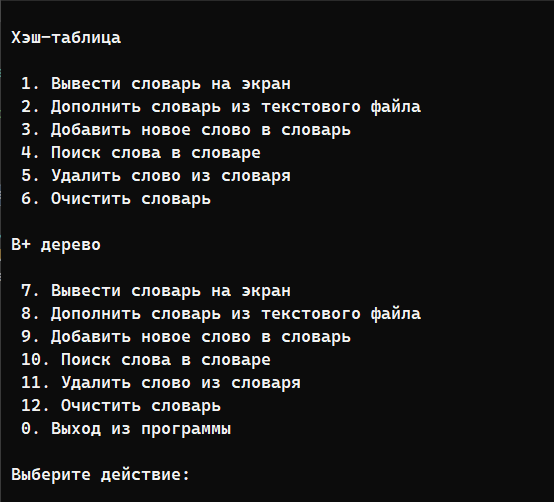
\includegraphics[width=0.5\linewidth]{img/pic3.png}
	\caption{Меню программы}
	\label{fig:pic3}
\end{figure}

При нажатии на клавишу один в самом начале программы, пользователю будет выведено сообщение о том, что хеш-таблица пуста. (\hyperref[fig:pic4]{рис.7}). \par

\begin{figure}[H]
	\centering
	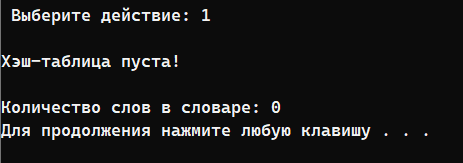
\includegraphics[width=0.5\linewidth]{img/pic4.png}
	\caption{Хеш-таблица}
	\label{fig:pic4}
\end{figure}


При нажатии на клавишу "2"\ в словарь будут добавлены слова из файла "story.txt", расположенного в корне проекта. После этого будет выведено информационное письмо пользователю о проведённой операции. (\hyperref[fig:pic5]{рис.8})

\begin{figure}[H]
	\centering
	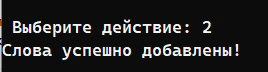
\includegraphics[width=0.35\linewidth]{img/pic5.png}
	\caption{Дополнение словаря из текстового файла}
	\label{fig:pic5}
\end{figure}


При нажатии на клавишу "3"\ пользователю будет предложено ввести слово, которое он хотел бы добавить в словарь. После ввода слова, выводится информация об успешности добавления слова в словарь. (\hyperref[fig:pic6]{рис.9})
\begin{figure}[H]
	\centering
	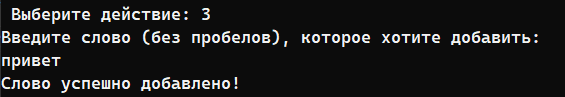
\includegraphics[width=0.45\linewidth]{img/pic6.png}
	\caption{Добавление нового слова в словарь}
	\label{fig:pic6}
\end{figure}


При нажатии на клавишу "4"\ пользователю будет предложено ввести слово, которое он хотел бы найти в словаре. После ввода слова, выводится информация об успешности поиска слова в словаре, а также в случае успеха будет выведен номер индекса массива хеш-таблицы, где расположено слово.  (\hyperref[fig:pic7]{рис.10})
\begin{figure}[H]
	\centering
	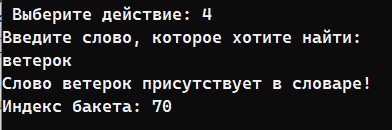
\includegraphics[width=0.45\linewidth]{img/pic7.png}
	\caption{Поиск слова в словаре}
	\label{fig:pic7}
\end{figure}

При нажатии на клавишу "5"\ пользователю будет предложено ввести слово, которое он хотел бы удалить из словаря. После ввода слова, выводится информация об успешности удаления слова из словаря. (\hyperref[fig:pic8]{рис.11})
\begin{figure}[H]
	\centering
	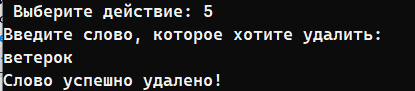
\includegraphics[width=0.45\linewidth]{img/pic8.png}
	\caption{Удаление слова из словаря}
	\label{fig:pic8}
\end{figure}

При нажатии на клавишу "6"\ словарь будет очищен. Также будет выведено соответствующее сообщение. (\hyperref[fig:pic9]{рис.12})
\begin{figure}[H]
	\centering
	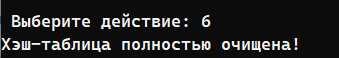
\includegraphics[width=0.45\linewidth]{img/pic9.png}
	\caption{Очистка хеш-таблицы}
	\label{fig:pic9}
\end{figure}


Помимо хеш-таблицы, в программе также присутствует возможность работы с B+-деревом. При нажатии на клавишу "7"\, отвечающую за отображение B+-дерева, при отсутствии в нём каких-либо элементов, будет выведено сообщение о том, что оно пустое. (\hyperref[fig:pic10]{рис.13})
\begin{figure}[H]
	\centering
	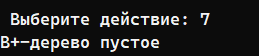
\includegraphics[width=0.35\linewidth]{img/pic10.png}
	\caption{Вывод пустого B+-дерева на экран}
	\label{fig:pic10}
\end{figure}

Работа клавиши "8"\ (дополнение словаря из текстового файла) аналогична работе клавиши "2"\ . (\hyperref[fig:pic11]{рис.14})
\begin{figure}[H]
	\centering
	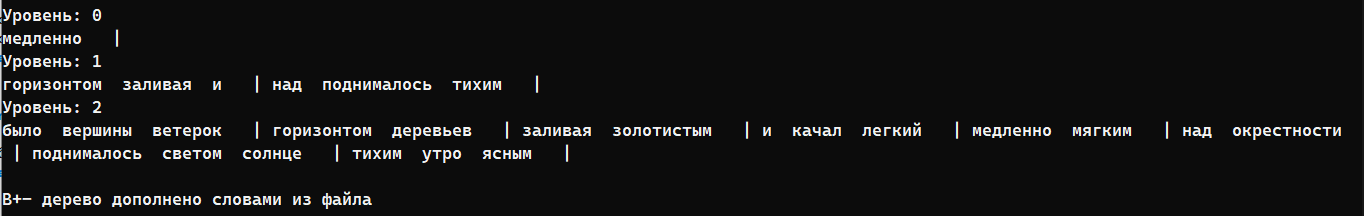
\includegraphics[width=0.9\linewidth]{img/pic11.png}
	\caption{Дополнение словаря из текстового файла}
	\label{fig:pic11}
\end{figure}


Работа клавиши "9"\ (вставки) аналогична работе клавиши "3"\ . (\hyperref[fig:pic12]{рис.15})
\begin{figure}[H]
	\centering
	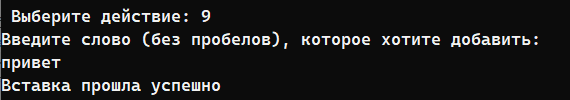
\includegraphics[width=0.8\linewidth]{img/pic12.png}
	\caption{Вставка нового слова в B+-дерево}
	\label{fig:pic12}
\end{figure}

Работа клавиши "10"\ (поиска) аналогична работе клавиши "4"\ . (\hyperref[fig:pic13]{рис.16})
\begin{figure}[H]
	\centering
	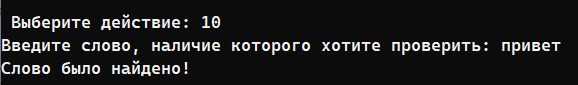
\includegraphics[width=0.8\linewidth]{img/pic13.png}
	\caption{Поиск слова в словаре}
	\label{fig:pic13}
\end{figure}
 
Работа клавиши "11"\ (удаления) аналогична работе клавиши "5"\ . (\hyperref[fig:pic14]{рис.17})
\begin{figure}[H]
	\centering
	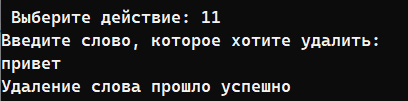
\includegraphics[width=0.6\linewidth]{img/pic14.png}
	\caption{Удаление слова из словаря}
	\label{fig:pic14}
\end{figure}

Работа клавиши "12"\ (очистка словаря) аналогична работе клавиши "6"\ . (\hyperref[fig:pic15]{рис.18})
\begin{figure}[H]
	\centering
	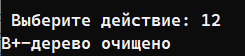
\includegraphics[width=0.4\linewidth]{img/pic15.png}
	\caption{Очистка словаря}
	\label{fig:pic15}
\end{figure}


\newpage
Также на рисунках 19-21 представлены некоторые исключительные ситуации, которые обрабатываются программой.
\begin{figure}[H]
	\centering
	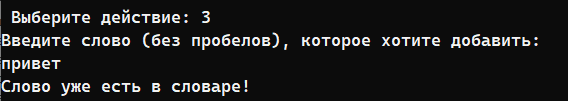
\includegraphics[width=0.5\linewidth]{img/pic16.png}
	\caption{Слово уже присутствует в словаре}
	\label{fig:pic16}
\end{figure}

\begin{figure}[H]
	\centering
	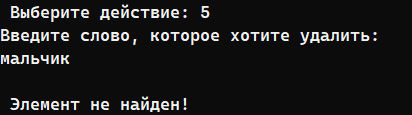
\includegraphics[width=0.5\linewidth]{img/pic17.png}
	\caption{Удаление несуществующего слова}
	\label{fig:pic17}
\end{figure}

\begin{figure}[H]
	\centering
	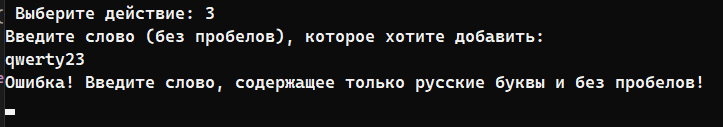
\includegraphics[width=0.6\linewidth]{img/pic18.png}
	\caption{Ввод слова, используя буквы не русского алфавита}
	\label{fig:pic18}
\end{figure}



\newpage
\section*{\hspace{1.15cm}Заключение}
\addcontentsline{toc}{section}{Заключение}

\setlength{\parindent}{1.2cm}
В ходе выполнения лабораторной работы был реализован словарь в двух вариантах: хеш-таблицей и B+-деревом. Для каждого из вариантов словаря были реализованы операции добавления, удаления и поиска, а также функции очистки словаря и загрузки/дополнения словаря из текстового файла. Для разрешения коллизий в хеш-таблице был использован метод цепочек. В качестве хеш-функции использовался полиномиальный хеш. \par
Хеш-функция, используемая в хеш-таблице генерирует значения от 0 до 10, за счёт такого небольшого диапазона она имеет значительно меньшую устойчивость к коллизиям, по сравнению с реализациями, в которых ширина диапазона значений достигает $2^{30}$ и более. Однако, чтобы уменьшить количество коллизий была введена переменная - \textbf{коэффициент заполнения}, которая представляет из себя отношение количества элементов в хеш-таблице к общему количеству бакетов. Когда коэффициент заполнения превышает определённый порог (0.75), происходит \textbf{рехеширование} — процесс, при котором создаётся новый массив большего размера с удвоенным количеством бакетов, и все существующие пары из старого массива переносятся в новый, с пересчётом индексов на основе новой хеш-функции. 

Из достоинств реализованной программы можно назвать наличие функции рехеширования, которая предотвращает появление большого числа коллизий при увеличении количества добавляемых слов, а также рассмотрение всех ситуаций при реализации операций добавления и удаления слова из словаря, основанного на B+-дереве. Также за счёт объектно-ориентированного подхода и разбиения кода B+-дерева на функции достигается высокий уровень его читаемости.\par

Недостатком реализованной программы является недоработка с подменой ссылок в корневом узле при удалении оттуда элемента. \par

В планы на масштабирование программы можно записать следующее:
\begin{enumerate}
	\item Реализация поиска однокоренных слов в хеш-таблице.
	\item Реализация бинарного поиска в узлах B+-дерева.
\end{enumerate}

\newpage
\addcontentsline{toc}{section}{Список использованной литературы}
\begin{thebibliography}{0}
	\bibitem{tema} Секция <<Телематика>>. - Текст: электронный // tema.spbstu.ru : [сайт]. - URL: \href{https://tema.spbstu.ru/tgraph/}{https://tema.spbstu.ru/tgraph/} (дата обращения 12.05.2024).
	\bibitem{novikov}  Новиков, Ф.А. ДИСКРЕТНАЯ МАТЕМАТИКА ДЛЯ ПРОГРАММИСТОВ Ф.А. Новиков. - 3-е издание. - Питер : Питер Пресс, 2009. - 384 с.
\end{thebibliography}

\end{document}